\chapter{实验与分析评测}\label{sec:experiment}
本章将针对水下图像多模态翻译问题设计实验、确定评价指标,验证我们设计的网络模块的有效性,并与基准方法进行对比和分析。

\section{水下图像跨域多模态合成实验设计}
\subsection{实验设置}
基准方法我们总共选取了五种,其中两种经典的图像翻译方法CycleGAN~\citep{zhu2017unpaired}和基于分解表示的跨域多模态翻译方法MUNIT~\citep{huang2018multimodal},三种最新的图像多模态翻译方法DRIT++~\citep{lee2020drit++}、DSMAP~\citep{chang2020domain}和StarGAN v2~\cite{choi2020stargan}。除了不可或缺的经典模型CycleGAN,剩余四种方法都可以完成两个域之间的多模态翻译任务。

CycleGAN学习两个域之间的一对一映射,通过循环一致性损失能够很好的学习到目标域的特征;MUNIT, DRIT++和DSMAP这些基于分解表达的方法,都是将图像进行分解,拆分为域共享的内容空间和不同域的特征空间,然后通过给生成器共享的内容和目标域的特征,合成与目标域风格相同的结果;StarGAN v2使用一个生成器结构,通过编码控制生成具有多个特征的多个目标域。在此,StarGAN v2用两个域之间的翻译来实验。

在我们的实验中,将$A$域设置为空中域,$B$域设置为多模态水下域,在以上五种基准方法上进行多个数据集的客观实验。在真实水下数据集和合成数据集上设置了针对模糊程度、水类型、以及特定水质状态的多个实验。

\subsection{数据集设置}
由于真实水下场景的配对数据集数量有限,在水下视觉工作中也常用合成水下数据集进行研究。常用的真实数据集和合成水下数据集有如下几种,在我们实验中,根据实验设计将数据集组合进行使用,以达到训练目的。

RUIE~\cite{liu2019real}是共有四千多张图像的大规模真实水下数据集。RUIE中包含三个子集,第一个子集UIQS包含五种浑浊程度的水下图像,其中每种726张,可用来测试水下图像增强效果;第二个子集UCCS包含蓝色、绿色以及蓝绿色三种色偏的水下图像,每种100张,用来评估颜色校正算法的性能;第三个子集为UHTS,包含对扇贝、海参和海胆三种海洋生物的标注,每种100张,用于高级计算机视觉任务如分类和检测。

UIEB~\cite{li2019underwater}是数量大、场景多样且具有高质量参考图像的成对真实场景数据集。原始图像共有950张,采用12种图像增强方法来进行图像增强,针对每张原始图像有50个志愿者来选出令人满意的图像增强结果作为真值,最终形成890张具有参考图像配对的结果,令半数以上人不满意的60结果作为挑战图像没有真值。

像以上这种水下图像数据相比较于非水下场景(空中)图像数量非常少,进行水下视觉图像研究时,研究人员会按照任务需要将空中图像进行水下环境条件模拟,合成该输入对应环境下的水下图像。

UWCNN~\cite{li2020underwater}论文中提出从地面图像得到相应水下图像数据集。通过NYU-v2~\cite{silberman2012indoor} RGB-D室内数据集生成10种类型的水下图像。NYU-v2室内共1449张图像,其中选出1000张用于实验训练,剩下的449张用于测试模型有效性,数据集提供的10类水下图像也是共1449张图像。对于每张室内图像,根据生成的随机均匀全球大气光和深度(从0.5米到15米),每张图像生成5张水下图像。NYU-v2室内数据集中的图像作为ground truth(真图),和合成的水下图像(假图)配对。

EUVP~\cite{islam2020fast}是UGAN~\cite{fabbri2018enhancing}中提出数据集的基础上更加齐全的数据集。UGAN中,ground truth是真实的相对不失真的水下图像(真图),配对的是生成的失真的水下图像(假图)。从ImageNet中选择一些不失真的水下图像,组成X域,共6143张图像,再从ImageNet中选择一些有明显水下图像特点的水下图像,组成Y域,共1817张图像。用CycleGAN实现风格迁移,即将X域中不失真的图像转成Y域中失真水下图像的风格(主要是颜色的变化)。最终用于训练的图像对是将X域中的图像都翻译成失真水下图像。EUVP中,分为paired和unpaired两种。Paired文件夹中包含3个子文件夹:Underwater Dark、Underwater ImageNet和Underwater Scenes,其中Underwater Dark有5550个图像对,570张验证图像,共11670张;Underwater ImageNet有3700个图像对,1270个验证图像,共8670张图像;Underwater Scenes有2185个图像对,130个验证图像,共4500张图像。Unpaired:poor quality中有3195张,good quality中有3140张,validation中有330张,共6665张图像。

UVB 2017是一个模拟的图像和视频数据集,是我们实验室在大连用ZED和Kinect摄像机进行拍摄的。用浓度不同的\ce{Al(OH)3}来模拟不同水质类型的衰减系数,摄像机收集了目标物在不同水质下的各种结果。已整理好的数据文件包括衰减为0即无水环境下的采集结果、衰减为1.2、1.58至衰减系数为3的多种结果。数据集在浑浊程度上随着衰减系数增加有视觉可见的从清晰到浑浊的变化过程。


由于水下环境导致采集数据受限,我们的数据集并不是十分充足,因此在一种实验设置中用到多个数据集的组合。我们在水下图像多模态翻译任务中,主要使用到RUIE~\citep{liu2019real}, UWCNN~\citep{li2020underwater}, UVB 2017数据集。EUVP~\citep{islam2020fast}和UIEB~\citep{li2019underwater}数据集作为补充进行组合实验。其中RUIE,UIEB和EUVP部分数据集是真实世界水下图像,UWCNN和UVB 2017是合成图像。这些数据集在各个子集数量上并不都是均衡的,所以训练时对模型方法提出了较高的要求。

\begin{figure*}[htp]
    \centering
	\includegraphics[width=\textwidth]{figures/ruie-dataset.pdf}
	\caption{RUIE数据集多模态翻译示例。图片来自文献~\cite{liu2019real,islam2020fast}。}
	\label{fig:ruie_dataset}
\end{figure*}

RUIE数据集是一个真实世界获取到的水下不配对图像集。如图~\ref{fig:ruie_dataset}所示,当我们进行水下色偏和清晰度实验训练时,选择RUIE的子集UCCS的300张图片当作水下域,选取EUVP中300张无水子集作为空中域。进行测试实验时,选择EUVP中的100张无水图像作为空中域,测试训练模型,以获得水下多模态域的结果。

\begin{figure*}[htp]
    \centering
	\includegraphics[width=\textwidth]{figures/uwcnn-dataset.pdf}
	\caption{UWCNN数据集多模态翻译示例。图片来自文献~\cite{li2020underwater}。}
	\label{fig:uwcnn_dataset}
\end{figure*}

UWCNN数据集使用NYU-v2 RGB-D图像来合成深海和近海的十种水类型。基于水下衰减模型,多个衰减系数当作不同的水类型的控制变量。如图~\ref{fig:uwcnn_dataset}所示,当我们进行训练时,选择1200张衰减系数为0即无水域的图像,选择近海type-1,type-3,type-5,type-7作为水下多模态域,每种类型选取300张,这几种水下类型在视觉上有直观可见的区别,方便后续进行定性评价。进行测试时,选择无水域中249张图像进行测试。

\begin{figure*}[htp]
    \centering
	\includegraphics[width=\textwidth]{figures/uvb-dataset.pdf}
	\caption{UVB数据集多模态翻译示例。}
	\label{fig:uvb_dataset}
\end{figure*}

如图~\ref{fig:uvb_dataset}所示训练时,UVB 2017数据集我们选择了660张图像作为无水域,447张不同深度和浑浊度的图像作为水下多模态域。测试时,无水域选取66张图像进行测试。

\subsection{评价准则}
为了方便对各个方法进行客观对比,在图像翻译角度从翻译结果真实性、多样性来进行评价。

\textbf{真实性。}真实性是指给定源域图像作为输入,生成的结果应该与目标域中的分布尽可能的相同。在我们的实验中,生成的水下多模态域结果应该在质量真实性评价上尽可能与真实样本分布相近。

我们在实验中,真实性指标选取Fréchet Inception Distance(FID)~\cite{heusel2017gans}来进行评价。基于Inception score~\cite{salimans2016improved}改进,FID最初由Heusel等人~\cite{heusel2017gans}提出。FID进行评价时,与Inception score一般,使用同样的Inception v3模型进行计算。
% 与Inception分数一样,FID分数也使用了Inception v3模型。具体而言,模型的编码层(图像的分类输出之前的最后池化层)被用来抽取输入图像的特征。使用来自Inception v3模型的激活函数的输出来归纳每个图像,得分即为Frechet Inception Distance。
FID能够完善Inception score没有比较模型生成样本和真实样本统计特性的问题。FID越低表示测评的图像质量越好,意味着生成图片跟真实结果之间相似性较高;反之,得分越高表示测评的图像质量越差,图像质量和指标结果呈现线性关系。

\textbf{多样性。}非成对图像多模态翻译问题中,在输入唯一时,能产生目标域的多模态结果。在水下图像多模态翻译任务中,当输入一张空中图像时,我们希望能得到多个对应的水下域图像翻译结果。即使都是相同的内容,在水质等水下条件不同时将导致水下图像的模态不一致。对于生成的多种图像,都能跟输入图像拥有相同的内容,再对生成结果进行多样性的评价。

在实验中,我们选用Learned Perceptual Image Patch Similarity (LPIPS)~\cite{zhang2018perceptual}来评价多样性指标。LPIPS最初由Zhang等人~\cite{zhang2018perceptual}提出,相比于传统的图像相似度评价指标,LPIPS指标得到的结果和人的视觉评价有更高的相关性。LPIPS用来评价生成结果的多样性,用预训练好的AlexNet~\cite{krizhevsky2017imagenet}网络来提取特征后计算L1距离。对于每个测试图像,用指定数量的随机采样向量来成指定数量的输出结果,对于同一个输入的多个结果对之间计算平均距离,最后计算所有测试输入的均值,并把这个数值当作LPIPS结果。

\textbf{水下质量评价。}
我们选取UCIQE~\cite{yang2015underwater}和UIQM~\cite{panetta2015human}作为我们实验中的水下图像评价指标,这两个指标是水下任务中评价水下图像质量的关键性指标。在进行测评时,不需要配对结果一起参与评价,属于无参考指标。
% 是无参考/无真值评价水下图像质量的常用指标,也是评价水下图像质量的关键指标。

UCIQE是色彩浓度、饱和度和对比度为测量分量的线性组合,可以定量的评价水下增强结果的色偏、模糊和对比度情况。首先将水下图像从RGB颜色空间转换到CIELab颜色空间,这样更符合人类视觉感知,然后计算各个测量分量,具体计算如式~\ref{equ:uciqe}所示。
\begin{equation}
\label{equ:uciqe}
UCIQE = c_1 \times \sigma_c + c_2 \times con_l + c_3 \times \mu_s
\end{equation}

其中,$ \sigma_c$为色度的标准方差,$con_l$为亮度的对比度,$\mu_s$是饱和度的平均值,$c_1$,$c_2$和$c_3$分别为线性组合的权重值。

UIQM针对水下图像的退化机理和成像特点,采用色彩测量UICM,清晰度测量UISM和对比度测量UIConM作为评价水下图像质量的依据。UIQM属于无参考/无真值的图像评价指标,通过测量分量的线性组合来表征图像的视觉质量,如式~\ref{equ:uiqm}所示。
\begin{equation}
\label{equ:uiqm}
UIQM = c_1 \times UICM + c_2 \times UISM + c_3 \times UIConM
\end{equation}

其中,$c_1$,$c_2$和$c_3$分别为线性组合的权重值。
% ,权重值的设定需要视具体任务而定,评价水下图像的颜色偏差修正结果时,需设定色度测量分量UICM更大的权重因子;当评价对比度和清晰度时,需要设定清晰度测量分量UISM和对比度测量分量UIConM更大的权重因子。

\section{水下图像跨域多模态合成结果分析}
\subsection{定性结果分析}

\begin{figure}
    \centering
	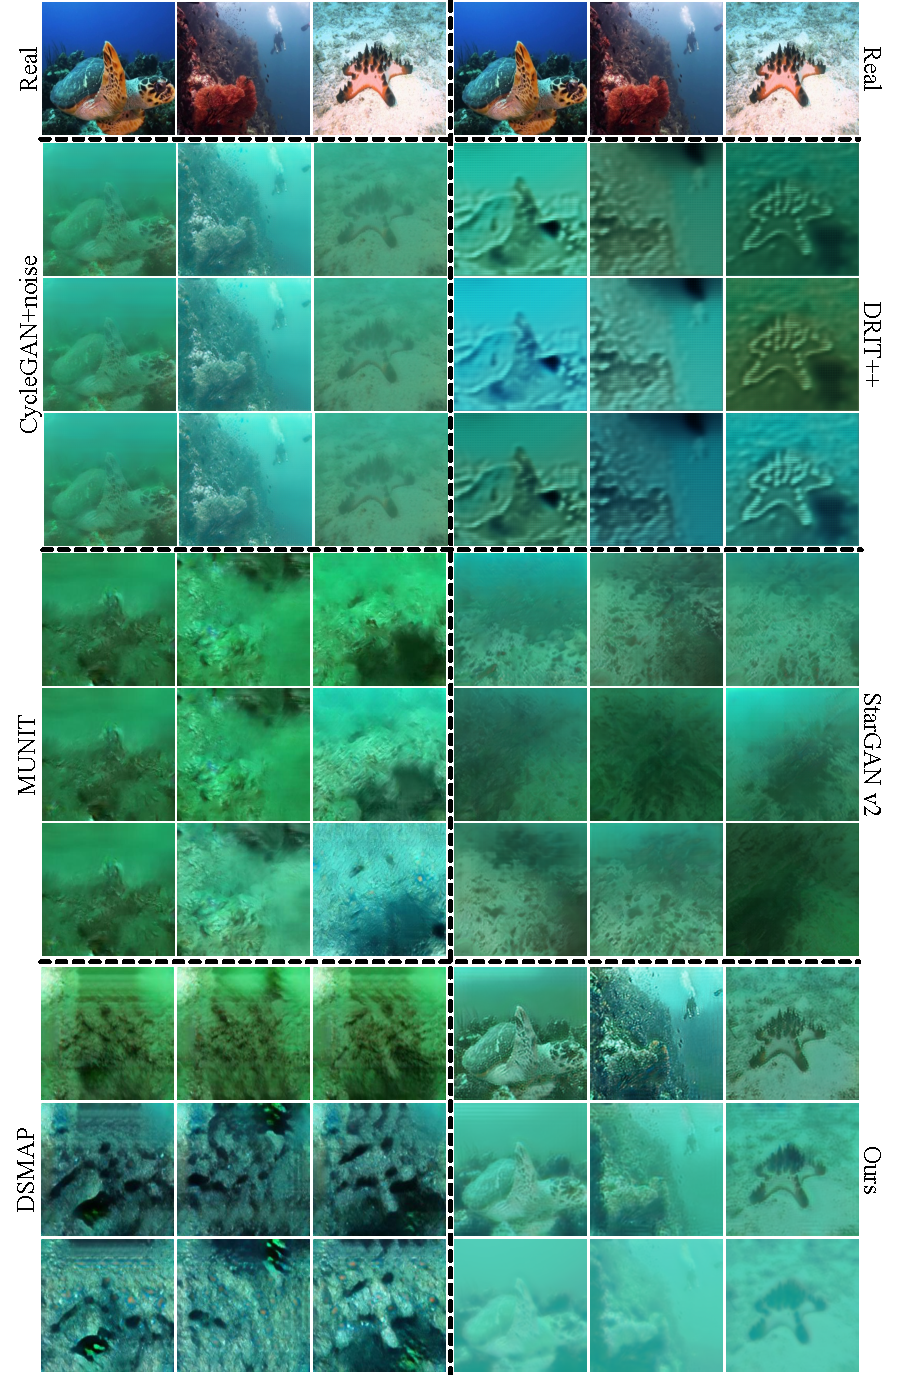
\includegraphics[width=\textwidth]{figures/RUIE_random_1.pdf}
	\caption{在RUIE数据集上,基准方法和我们提出的方法在目标域随机采样生成的多模态结果比较。}
	\label{fig:ruie_random_1}
\end{figure}

\begin{figure}
    \centering
	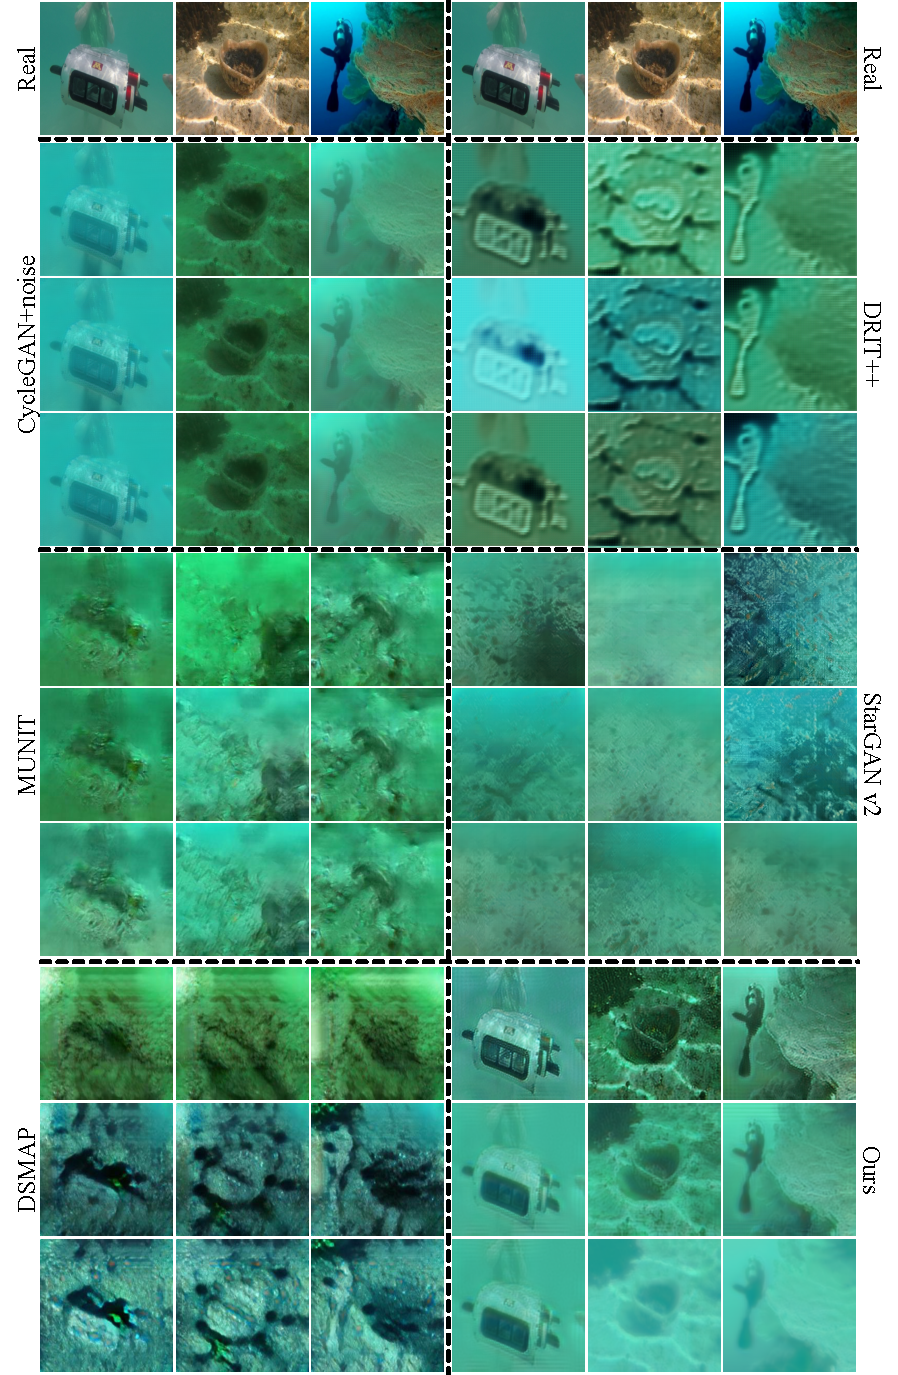
\includegraphics[width=\textwidth]{figures/RUIE_random_2.pdf}
	\caption{在RUIE数据集上,基准方法和我们提出的方法在目标域随机采样生成的多模态结果比较。}
	\label{fig:ruie_random_2}
\end{figure}

图~\ref{fig:ruie_random_1}和图~\ref{fig:ruie_random_2}展示了基准方法和我们方法在RUIE数据集上的定性对比结果。第一行Real表示模型输入图像,之后每行都是对应标记方法获得的结果。从对比图中可以看到,CycleGAN+noise方法的翻译结果比较真实,内容信息保留完整,但是噪声被忽略,每行加入不同的风格采样信息单没有多模态样式的结果;MUNIT方法翻译结果质量较差,轮廓信息几乎全部丢失,尽管模态之间能看出区别,从行结果上看同样的风格采样信息影响的风格样式并没有一致;DSMAP方法中每行风格信息影响的样式上能看出一致的差异,很明显内容和风格也没有分解彻底,DSMAP的内容受风格样式的影响很严重,保留较少内容细节留,可以看出DSMAP对于内容的处理非常粗糙,生成结果边缘也有伪影的出现。DRIT++方法的结果,内容轮廓能够得到有效的保留,内容细节丢失十分严重,DRIT++有多模态效果,但每行模态没有没有实现一致的效果;StarGAN v2方法生成的结果很差,视觉上是学习到了海底样式,但是内容没有有效保留并控制模态样式变化,通过训练没有成功学习并实现我们想要的多模态翻译任务。而本文提出的多模态翻译方法,简洁有效地将内容信息和风格信息进行分解,在内容上,能够极好地保留目标物和水纹理等轮廓信息和目标颜色变化等细节信息,在风格上,每行相同风格信息输入能够实现每行风格样式结果的一致,定性视觉上,真实有效地实现水下图像多模态的合成。

\begin{figure}
    \centering
	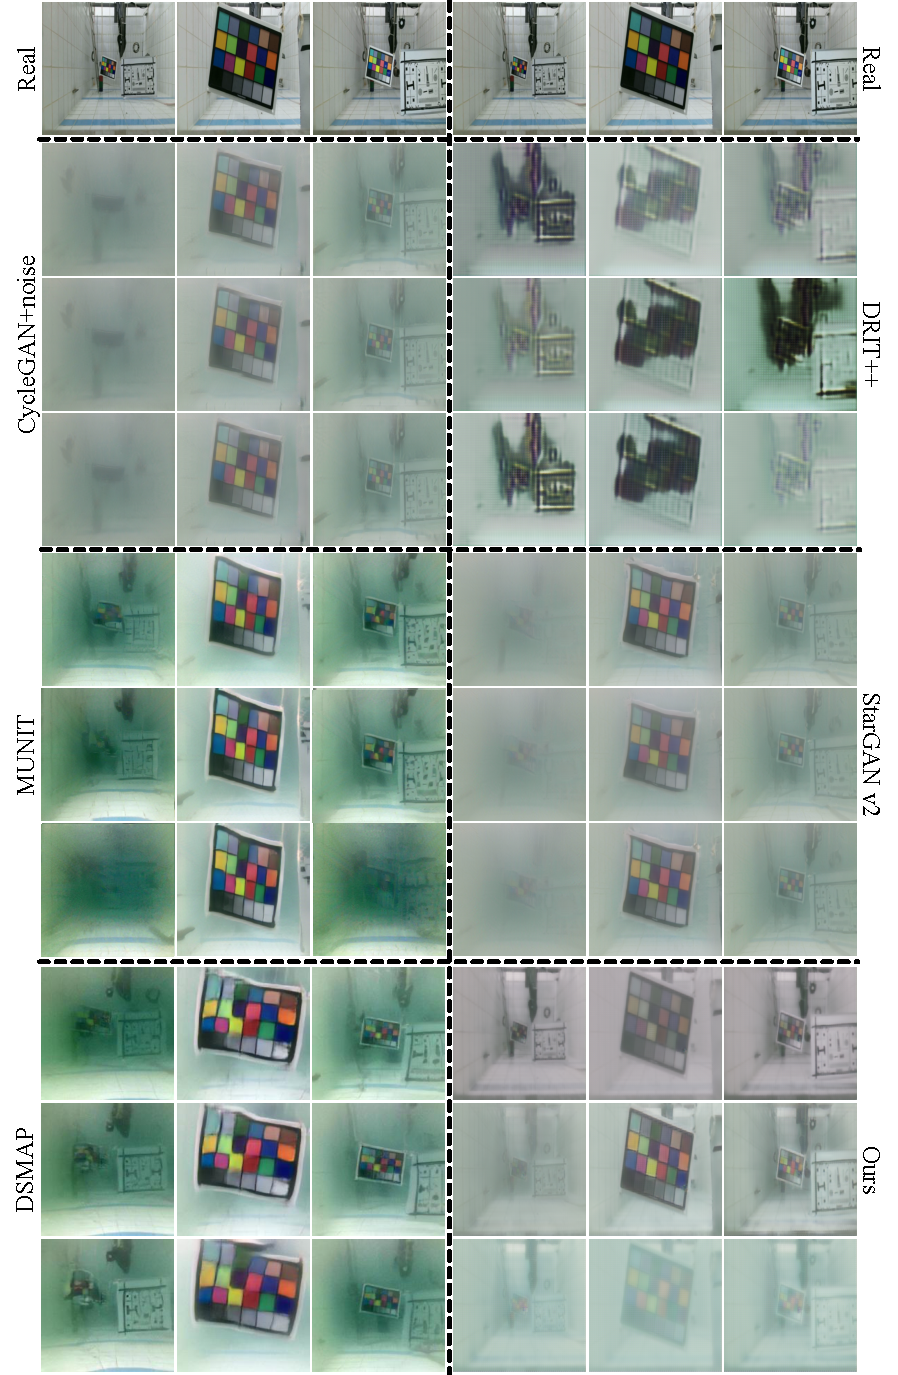
\includegraphics[width=\textwidth]{figures/UVB_random.pdf}
	\caption{在UVB 2017数据集上,基准方法和我们提出的方法在目标域随机采样生成的多模态结果比较。}
	\label{fig:uvb_random}
\end{figure}

图~\ref{fig:uvb_random}展示了基准方法和我们方法在UVB 2017数据集上的定性结果对比。对比图中第一行Real指示模型输入图像,之后每行都是对应标记方法获得的结果。从对比图中可以看到,CycleGAN+noise方法的翻译结果较为真实,在浑浊度变化的UVB 2017数据集上尽管内容保持较为完整,像色卡这种比较直观的目标物可以看出翻译结果在色卡颜色上保留较好,但是色卡轮廓发生了扭曲,而且没有模态上的变化,噪声对于模态的影响在肉眼上无法辨别;MUNIT方法翻译结果内容上可以较好的保留,在目标物轮廓上依旧会发生形变,导致目标物视觉上扭曲,在风格样式上,对于较近的目标物,浑浊程度的变化不明显,对于较远的目标物,能够明显看出浑浊程度在不同模态样式上发生了变化;DSMAP方法翻译结果类似MUNIT翻译结果,目标物在内容上会发生形变,在色卡各个颜色之间的扭曲会比MUNIT更明显,整体可保留一定内容;DRIT++方法翻译结果,内容上不能保留让人满意的结果,对于内容轮廓能够很好的进行保留,但是对于内容细节,保留不完整,颜色比较复杂的部分接被黑色阴影填充,导致内容没有完整保留,风格固定均为白色模糊,并会出现棋盘网格样式,推断是网络结构设计导致的问题;StarGAN v2方法在UVB 2017数据集上能生成比RUIE真实水下数据集明显成功的翻译结果,可以看出StarGAN v2对于数据集本身有一定的要求,在UVB 2017数据集上,内容可以基本保留完整,在色卡上可以看出有轻微的扭曲变形,但是颜色基本保持完整,对于远处的目标物形状基本也完整,风格样式上,视觉效果不明显,多行之间无法清楚辨认出是来自不同模态的结果。而本文提出的水下图像多模态翻译方法,内容能够几乎全部被完整保留,不论位置较近还是较远的目标物颜色都没有发生改变,仅有模态导致的一定程度模糊,形状无扭曲,三个模态的三行结果可以明显看出有样式上的区别,且每个模态影响的风格样式都保持了不同目标上的一致性。可以明显的看出我们的模型在UVB 2017数据集上也可以展现较好的效果。

\begin{figure}
    \centering
	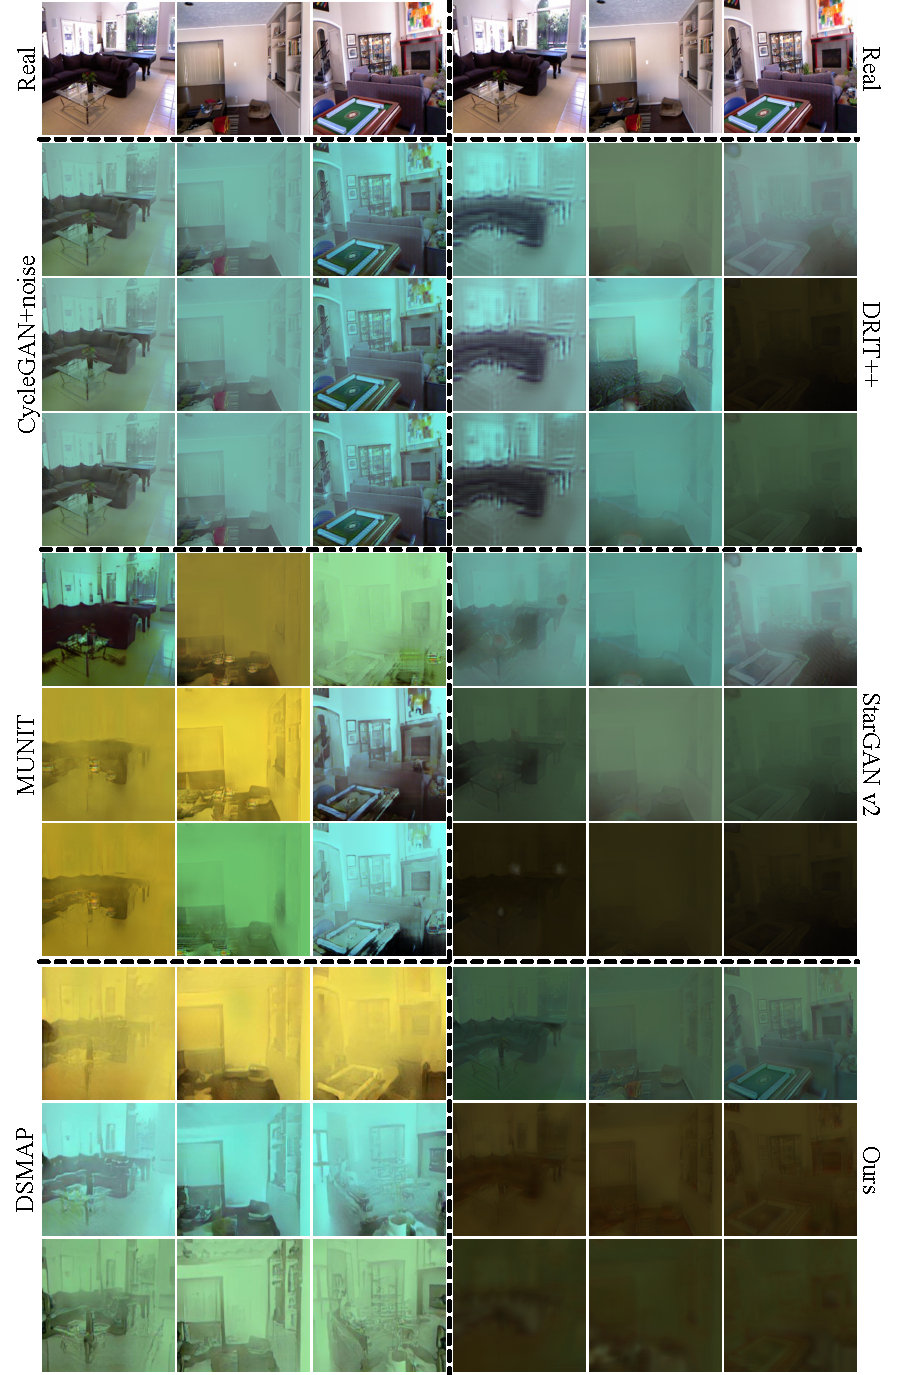
\includegraphics[width=\textwidth]{figures/UWCNN_random.pdf}
	\caption{在UWCNN数据集上,基准方法和我们提出的方法在目标域随机采样生成的多模态结果比较。}
	\label{fig:uwcnn_random}
\end{figure}

图~\ref{fig:uwcnn_random}展示了不同方法在UWCNN数据集上的定性结果对比。第一行Real表示模型输入图像,之后每行都是对应标记方法获得的结果。CycleGAN+noise方法的翻译结果真实度较高,对于输入图像中的内容保存完好,可以看出生成结果不存在多模态样式,且噪声被模型忽略,无法扰动生成网络从而合成多模态结果;MUNIT在UWCNN数据集上生成的结果较为真实,内容也保存比较完好,但是在生成结果中,色彩较多的部分(如图~\ref{fig:uwcnn_random} MUNIT生成结果中茶几上的部分)会出现翻译失败的情况,生成结果能出现多模态效果,但每行同一种风格样式编码无法控制模态一致性;在MUNIT方法上进行改进的DSMAP方法翻译效果有明显的提升,在内容上基本保留完整,细节处有轻微变形,图像中的物体轮廓发生了扭曲,对于每行同样的风格编码输入,能有整齐一致的模态变化,在风格上的翻译十分成功,但内容没有保持原有的形态;DRIT++方法翻译结果,部分内容损失严重,其中轮廓变得模糊,没有清晰的边界,对于雾较为浓厚的模态这种问题不明显,对于雾轻薄的地方,内容的损失就很清晰的展现出来,风格上能有多模态样式,对于每行同一风格编码输入,不能合成一致的模态样式;StarGAN v2结果基本内容能够保存完整,除了内容轮廓有轻微扭曲,整体内容较为完整,且雾与数据集中展示的距离越远的地方雾越厚一致,风格上能生成多模态效果,每行模态效果相似,但不能完全一致,整体风格能看出多模态效果。本文提出的方法在内容上保存完整,无论是内容细节还是内容轮廓都没有发生变化,颜色信息也能在合成过程中保留,对于每行不同的风格编码,每行能有一致的风格样式,且模态间有明显区别的多模态结果。本文提出的方法不仅对于真实水下图像,对于合成水下图像一样能进行有效的多模态控制。

\begin{figure*}[ht]
    \centering
	\includegraphics[width=\textwidth]{figures/RUIE_guidance.pdf}
	\caption{RUIE数据集上,本文提出方法用参考图像引导生成指定模态的结果。}
	\label{fig:ruie_guide}
\end{figure*}

图~\ref{fig:ruie_guide}展示了本文提出方法在参考图像引导方式上的多模态结果。对于输入图像,我们给出明确的参考风格图像,将参考图像编码成可以被生成器获取到的风格编码,如此可以合成指定参考风格的结果。从每一列可以看出,输入图像的内容得到了很好的保留,细节和轮廓都没有发生任何损失,从每行可以看出,风格影响的水质和模糊程度在不同输入图像上也影响一致。这说明,本文提出的方法能够有效的将图像中的内容和风格进行分解,内容信息作为恒定不变的部分,在翻译过程中需要完整的保留,风格信息作为模态的控制变量,在翻译时,源风格信息要彻底清除,且被目标风格带入翻译过程。

\begin{figure*}[ht]
    \centering
	\includegraphics[width=\textwidth]{figures/UVB-change.pdf}
	\caption{在UVB 2017数据集上,浑浊程度样式逐步变化过程。}
	\label{fig:uvb-change}
\end{figure*}

图~\ref{fig:uvb-change}展示了本文提出方法在UVB 2017数据集模态逐步变化的效果。图中Real A代表输入图像,Real B代表目标图像,中间为模态生成结果。我们的方法除了如图~\ref{fig:ruie_guide}中展示的让输入图像A生成目标图像B模态下的结果外,还可以合成逐步从模态A样式变化至模态B样式的结果。A是水下没有浑浊的图像,B是水下浑浊明显的图像,从生成的结果中可以看到,生成图像从左往右依次变化过程中,浑浊度不断增加,趋向于B中浑浊程度。在生成结果中,模态逐步变化,图像中的内容保持不变,仅仅是浑浊程度这个样式上发生了改变,内容的颜色、细节和轮廓都保存完整。

\subsection{定量结果分析}

真实性和多样性定量指标如表~\ref{tab:ruie_comparison}、~\ref{tab:uvb_comparison}和~\ref{tab:uwcnn_comparison}所示。根据定量结果分析中,我们对比了CycleGAN、MUNIT、DRIT++、DSMAP、StarGAN v2基准方法在RUIE、UVB 2017和UWCNN数据集上的实验评价。

\begin{table*}[ht]
\centering
\caption{在RUIE数据集上,基准方法和我们方法的真实性和多样性定量比较。}
  \begin{tabular}{c|ccccccccc}
    \hline\noalign{\smallskip}
    方法 & CycleGAN+noise & MUNIT & DRIT++ & DSMAP & StarGAN v2 & Ours \\
    \noalign{\smallskip}\hline\noalign{\smallskip}
    FID$\downarrow$ & 143.4 & 139.4 & 179.2 & 139.6 & 121.1 & \textbf{83.2} \\
    LPIPS$\uparrow$ & 0.534 & 0.452 & 0.575 & 0.513 & 0.431 & \textbf{0.579} \\
    \noalign{\smallskip}\hline
  \end{tabular}
  \label{tab:ruie_comparison}
\end{table*}

从表格~\ref{tab:ruie_comparison}中我们可以看到,在真实水下获取到的RUIE数据集上从空中到水下多模态域翻译的定量结果对比。CycleGAN+noise方法评价中,FID指标较高,说明跟真实水下图像差距较大,分析原因主要是因为CycleGAN+noise生成结果较为固定,跟真实多模态样本之间会存在较大的差异,输入图像的合成结果加上噪声也没有多模态样式,但是自身翻译结果是真实样本多模态样式中的任意一种,在计算LPIPS指标时,结果看起来令人满意,实际上同一输入无法产生多模态结果;MUNIT方法评价中,FID指标较高,说明跟真实水下图像差距较大,这主要是由于合成结果中内容损失严重,内容在轮廓上都无法与模态样式分离,在计算LPIPS指标时,能生成多模态效果但是模态之间效果差别较小,多样性不够导致LPIPS指标较低;DRIT++方法评价中,由于合成的结果内容细节信息丢失严重,在与真实样本计算FID指标时,必然会有巨大的差距,所以FID指标最高,真实性最差,在计算LPIPS指标时,对于不同的风格采样,同一输入可以生成不同模态的结果,因此多样性足够高,可以看出与我们方法指标相差无几,但是对于每种特定的风格采样,不同输入无法生成一致模态的结果;DSMAP方法是在MUNIT方法上进行改进,将域共享内容信息分解出域特有的内容信息,实际上将内容和风格进一步分解,这样获得到的内容信息更加纯净,在测量指标时,由于合成结果内容损失严重,除了部分轮廓能辨认其余内容信息全部丢失,在计算FID时,跟真实样本结果之间的差异巨大,导致FID指标较高,在计算LPIPS指标时,输入每种模态风格能有一致的合成模态结果,因此多样性存在;StarGAN v2方法中,由于生成结果内容没有有效保留,但是学习到了海底样式,所以在评价FID指标时,结果略高,存在多模态效果但是模态之间差异不明显,在评价LPIPS指标时结果较低,多样性不足。对本文中提出的方法进行评价,生成结果内容保留完好,且合成结果接近真实样本,所以FID结果较低,说明合成结果真实性高;能够通过对目标域风格随机采样或者通过参考图像进行引导合成真实的多模态结果,有足够多的模态样式,所以LPIPS指标最高,说明合成结果多样性充足。

\begin{table*}[ht]
\centering
\caption{在UWCNN数据集上,基准方法和我们方法的真实性和多样性定量比较。}
  \begin{tabular}{c|ccccccccc}
    \hline\noalign{\smallskip}
    方法 & CycleGAN+noise & MUNIT & DRIT++ & DSMAP & StarGAN v2 & Ours \\
    \noalign{\smallskip}\hline\noalign{\smallskip}
    FID$\downarrow$ & \textbf{80.7} & 232.1 & 290.7 & 138.8 & 149.8 & 129.6          \\
    LPIPS$\uparrow$ & 0.490         & 0.647 & 0.668 & 0.513 & 0.595 & \textbf{0.736} \\
    \noalign{\smallskip}\hline
  \end{tabular}
  \label{tab:uwcnn_comparison}
\end{table*}

从表格~\ref{tab:uwcnn_comparison}中我们可以看到,在合成数据集UWCNN空中到水下多模态图像域翻译的定量结果对比。CycleGAN+noise方法测评中,图像真实性非常高,跟数据集中部分真实样本分布接近,在计算FID时,CycleGAN+noise和真实数据之间的差距非常小,在计算LPIPS时,由于该方法合成的样本不受风格编码的扰动,合成样本的多样性缺乏,因此LPIPS指标较低;MUNIT方法测评中,图像内容可以较好的保留,目标物轮廓上依旧会发生形变,导致目标物视觉上扭曲,在计算FID时,差异较大,扭曲导致真实性下降,在计算LPIPS时,能看出模态在不同风格编码输入时发生变化,所以LPIPS指标较高,多样性结果存在;DSMAP方法测评中,类似MUNIT会发生形变,且扭曲比MUNIT更严重,所以在计算FID时结果值较高,真实性更低,在计算LPISP时,不同输入之间的多模态样式不明显,导致多样性不足,指标较低;DRIT++方法测评中,由于内容信息中复杂的部分被黑色阴影填充,真实性降低,因此FID指标最高,由于不同的模态样式编码输入可以影响合成不同样式,有多样性结果,因此LPIPS值较高;StarGAN v2在UWCNN数据集上可以合成视觉上真实的结果,与真实样本分布较为接近,因此FID较低,但是在风格上缺乏多模态合成结果,因此LPIPS也比较低。本文提出的方法在合成结果中,内容信息保留完整,在所有基于分解的翻译方法中FID最低,且有多种样式的合成结果,多样性足够所以LPIPS可以获得最高值。

\begin{table*}[ht]
\centering
\caption{在UVB数据集上,基准方法和我们方法的真实性和多样性定量比较。}
  \begin{tabular}{c|ccccccccc}
    \hline\noalign{\smallskip}
    方法 & CycleGAN+noise & MUNIT & DRIT++ & DSMAP & StarGAN v2 & Ours \\
    \noalign{\smallskip}\hline\noalign{\smallskip}
    FID$\downarrow$ & \textbf{145.1} & 240.4 & 243.7 & 232.6 & 162.9 & 172.7          \\
    LPIPS$\uparrow$ & 0.358          & 0.486 & 0.474 & 0.444 & 0.358 & \textbf{0.493} \\
    \noalign{\smallskip}\hline
  \end{tabular}
  \label{tab:uvb_comparison}
\end{table*}

从表格~\ref{tab:uvb_comparison}中我们可以看到,在合成数据集UVB 2017空中到水下多模态图像域翻译的定量结果对比。CycleGAN+noise方法测评中,翻译结果真实度较高,对于输入图像中的内容保存完好,在计算FID时,能够得到最低值,但是由于CycleGAN+noise生成结果不具有多样性,在计算LPIPS时结果较差;MUNIT生成的结果较为真实,内容也保存比较完好,会出现真实样本中不存在的黄色模态,且颜色较多的部分翻译会失败,在计算FID时,与真实结果差别较大,真实性不高,FID值很高,在计算LPIPS时会出现多种模态样式,且模态间差别很大,所以LPIPS指标较高;DSMAP在内容上基本保留完整,因为出现了真实样本中不存在的黄色模态结果,所以FID指标较高,缺乏真实性,合成结果能在模态上出现多样性且模态内的一致性,LPIPS指标结果较高;DRIT++方法测评中,轮廓模糊,边界不清晰,与真实样本结果区别较大,FID指标最高,真实性最低,尽管模态内结果不一致,但合成结果有明显的模态差异,LPIPS指标较高,具有多样性;StarGAN v2结果基本内容能够保存完整,且合成模态非常近似真实样本,FID指标较低,真实性较高,风格上生成的多模态效果模态内不稳定,LPIPS指标较低,多样性不充足。本文提出的方法测评中,内容上保存完整,在所有基于分解表达的方法中可以得到最好的FID结果,真实性较高;真实样本中存在的多种样式合成结果都有,多样性充足所以LPIPS最高。

\subsection{消融实验}

为了验证我们设计网络的有效性,主要对于生成器部分进行模块验证。通过使用MUNIT和DRIT++的生成器来验证我们生成器结构的有效性;通过对比有无内容一致性损失限制的结果,验证我们提出内容一致性限制的有效性。

\begin{table*}[htbp]
  \centering
  \caption{在RUIE、UVB 2017和UWCNN数据集上,生成器结构的比较结果。}
    \begin{tabular}{c|c|c|c|c|c|c}
    \hline
    \multirow{2}[3]{*}{} & \multicolumn{2}{c|}{MUNIT} & \multicolumn{2}{c|}{DRIT++} & \multicolumn{2}{c}{Ours} \\
\cmidrule{2-7}          & \multicolumn{1}{c|}{FID$\downarrow$ } & \multicolumn{1}{c|}{LPIPS$\uparrow$} & \multicolumn{1}{c|}{FID$\downarrow$ } & \multicolumn{1}{c|}{LPIPS$\uparrow$} & \multicolumn{1}{c|}{FID$\downarrow$ } & LPIPS$\uparrow$ \\
    \midrule
    RUIE  & 88.0388 & 0.438 & 92.2588 & 0.462 & \textbf{83.2399} & \textbf{0.579} \\
    UVB  & 197.7265 & 0.469 & 181.7613 & 0.489 & \textbf{172.7404} & \textbf{0.493} \\
    UWCNN & 185.4869 & 0.627 & 185.1982 & 0.598 & \textbf{129.6982} & \textbf{0.736} \\
    \hline
    \end{tabular}%
  \label{tab:comp_G}%
\end{table*}%

表格~\ref{tab:comp_G}所示为生成器有效性的验证结果。在相同的网络框架下,对比了基于分解表达方法MUNIT、DRIT++生成器,用真实性和多样性指标FID和LPIPS共同验证我们生成器结构的有效性。从表格中可以看出,我们生成器合成的水下图像多模态结果在真实性和多样性上都优于同样基于分解表达学习的经典方法MUNIT和DRIT++。FID是所有生成器生成结果中最低的,最接近真实样本分布,LPIPS是所有翻译结果中最高的,多样性丰富。

\begin{figure}
    \centering
  \includegraphics[width=\textwidth]{figures/Ablation_modal_ruie.pdf}
  \caption{RUIE数据集上,翻译器有效性对比结果。}
  \label{fig:ablation_modal_ruie}
\end{figure}

图~\ref{fig:ablation_modal_ruie}所示是RUIE数据集上本工作的生成器跟MUNIT、DRIT++生成器生成结果对比。在RUIE数据集上,我们对比了使用MUNIT、DRIT++生成器的生成结果。在多模态样式模糊程度和视觉效果任务下,MUNIT、DRIT++生成器在相同网络架构下,通过对目标域分布随机采样,生成多模态结果。其中各个方法都能成功生成多模态样式,在MUNIT和DRIT++中噪声对颜色样式造成影响十分明显。MUNIT方法中,内容损失很严重,在模态变化中,内容保存不完整,DRIT++中,内容能保留较为完整,但是三个模态中,颜色变化明显,针对模糊程度没有明显的变化。

\begin{table*}[htbp]
  \centering
  \caption{在RUIE、UVB 2017和UWCNN数据集上,生成器结构有无内容一致性限制结果。}
    \begin{tabular}{c|c|c|c|c|c|c}
    \hline
    \multirow{2}[3]{*}{} & \multicolumn{2}{c|}{RUIE} & \multicolumn{2}{c|}{UVB 2017} & \multicolumn{2}{c}{UWCNN} \\
\cmidrule{2-7}          & \multicolumn{1}{c|}{FID$\downarrow$ } & \multicolumn{1}{c|}{LPIPS$\uparrow$} & \multicolumn{1}{c|}{FID$\downarrow$ } & \multicolumn{1}{c|}{LPIPS$\uparrow$} & \multicolumn{1}{c|}{FID$\downarrow$ } & LPIPS$\uparrow$ \\
    \midrule
    Ours  & \textbf{83.2399} & \textbf{0.579} & \textbf{172.7404} & \textbf{0.493} & \textbf{129.6982} & \textbf{0.736} \\
    Ours w/o $\mathcal{L}_{cc}$ & 85.0344 & 0.575 & 175.3312 & 0.499 & 129.8680 & 0.724 \\
    \hline
    \end{tabular}%
  \label{tab:ablation_modal_lcc}%
\end{table*}%

表格~\ref{tab:ablation_modal_lcc}所示为生成器有无内容一致性损失$\mathcal{L}_{cc}$的对比结果,在RUIE、UVB 2017和UWCNN数据集上都进行了对比实验。在对比结果中我们可以看到,在有内容一致性损失$\mathcal{L}_{cc}$时,我们的结果在真实性和多样性上都有比较稳定的结果,当没有内容一致性损失$\mathcal{L}_{cc}$时,生成结果中的内容保留不如有内容一致性损失$\mathcal{L}_{cc}$的结果,所以FID较高,真实性不如有内容一致性损失$\mathcal{L}_{cc}$结果的真实性,但是在多样性上,内容一致性损失$\mathcal{L}_{cc}$对最终的结果影响不大,所以LPIPS结果接近。

\section{水下图像多种样式域合成实验设计}
\subsection{实验设置}
基准方法我们总共选择了三种,经典非配对跨域图像翻译方法CycleGAN~\cite{zhu2017unpaired},两种最新颖的多域翻译模型StarGAN v2~\cite{choi2020stargan}和MDMM~\cite{lee2020drit++}(DRIT++中拓展至多域翻译任务Github项目)。其中,跨域翻译模型CycleGAN可以学到两个域一对一的映射,在进行多域翻译时,需要域两两之间进行训练,无法一次同时实现多个域的训练。

CycleGAN可以看成两个GAN的融合,两个网络构成循环过程通过循环一致性损失,实现非配对的跨域翻译;MDMM依旧使用分解的方式,用一个生成器实现多个域的翻译,给定其中两个域的图像和one-hot编码,分解到共享内容空间和域特有风格空间,类似DRIT跨域翻译方式进行训练;StarGAN v2是在多域翻译模型StarGAN基础上的多域多模态翻译模型,StarGAN使用一个生成器网络输入源域图像和目标域的域标签,学习将图像从源域翻译到目标域,StarGAN v2将域标签替换成域特有风格编码来代表特定域风格的多种样式。

在我们的实验中,将源域图像翻译到$A$、$B$、$C$...等多种水下样式域,在以上三种基准方法上进行了多个数据集的实验。同样地,在真实水下数据集和合成数据集上设置了针对模糊程度、水颜色、以及特定水质状态的多个实验。

\subsection{数据集设置}
由于水下图像数据限制,在多域翻译任务中我们实验同样会用到多个数据集组合。在水下多种样式域翻译任务中,主要使用RUIE~\cite{liu2019real},UWCNN~\cite{li2020underwater},UVB 2017数据集,另外使用EUVP~\cite{islam2020fast},UIEB~\cite{li2019underwater}作为补充数据集,在实验中填补数据不充分的问题。

\begin{figure*}[ht]
    \centering
  \includegraphics[width=\textwidth]{figures/RUIE_dataset_domain.pdf}
  \caption{RUIE数据集多域翻译示例。图片来自文献~\cite{liu2019real,islam2020fast}。}
  \label{fig:ruie_domain}
\end{figure*}

如图~\ref{fig:ruie_domain}所示,RUIE数据集进行多种样式域翻译实验时,选择RUIE的子集UCCS的三种作为水下三个样式域,每种100张,选取EUVP中的100张图像作为空中域。在进行测试实验时,选择EUVP中无水域的100张作为空中域,测试训练模型,以测试模型翻译到水下多个样式域的效果。

\begin{figure*}[ht]
    \centering
  \includegraphics[width=\textwidth]{figures/UVB_dataset_domain.pdf}
  \caption{UVB 2017数据集多域翻译示例。}
  \label{fig:uvb_domain}
\end{figure*}

如图~\ref{fig:uvb_domain}所示,Underwater Vision Benchmark 2017(UVB 2017)数据集进行多种样式域翻译实验时,选择衰减为0中660张图像作为空中域,衰减为1.2、1.58、3.0四种样式明显的作为水下样式域。在进行测试时,选择无水中的30张图像测试模型翻译到多种样式域的效果。

\begin{figure*}[ht]
    \centering
  \includegraphics[width=\textwidth]{figures/UWCNN_dataset_domain.pdf}
  \caption{UWCNN数据集多域翻译示例。图片来自文献~\cite{li2020underwater}。}
  \label{fig:uwcnn_domain}
\end{figure*}

如图~\ref{tab:uwcnn_comparison}所示,UWCNN数据集进行多种样式域翻译实验时,选择室内图像中249张图像作为空中域,近海type-1,type-3,type-5,type-7四种较为明显样式的域作为水下多种样式域,每个域选择249张。测试时,选择100张图像进行测试。

\subsection{评价准则}
为了方便进行质量评价,我们对图像的真实性进行评价。真实性选用Fréchet Inception Distance(FID)来进行评价。FID比较模型生成样本和真实样本统计特性的问题。FID越低,图像质量越好;反之,得分越高,质量越差。较低的FID意味着两个分布之间更接近,也就意味着生成图片的跟真实结果之间相似性较高。在进行多种样式域实验中,我们生成的多个域结果与该域真实图像之间计算FID,就可以比较出每个域的生成结果与真实结果之间的相似性。

另外,还使用水下指标UCIQE和UIQM来验证生成结果的真实性。UCIQE和UIQM都是无参考批评家指标,当生成结果足够真实时,目标域的生成结果和真实样本在这两个指标在色彩、饱和度、对比度上,清晰度等质量上是一致的。通过对比真实样本和合成样本的评价结果,可以看出样本的真实性。

\section{水下图像多种样式域合成结果分析}
在翻译到不同视觉效果水下多种样式域任务中,CyleGAN无法实现多域之间翻译,实现需要两两之间组合训练,我们实验从输入到几个域的样式翻译,需要训练几次,保存几个翻译模型进行测试;MDMM是基于分解表达的多域翻译模型,将图像分解成共享的内容空间和特有的风格空间,多个域被编码作为条件输入网络结构,控制对应结果的生成;StarGAN v2是多域翻译模型StarGAN的最新多模态版本,在完成多域翻译任务时,我们将多模态样式设置为1,此时即可完成多域翻译任务。在本节中,我们对多个域翻译中的水质颜色、浑浊程度、视觉效果多种任务进行了大量实验。

\subsection{定性结果分析}
\begin{figure}
    \centering
  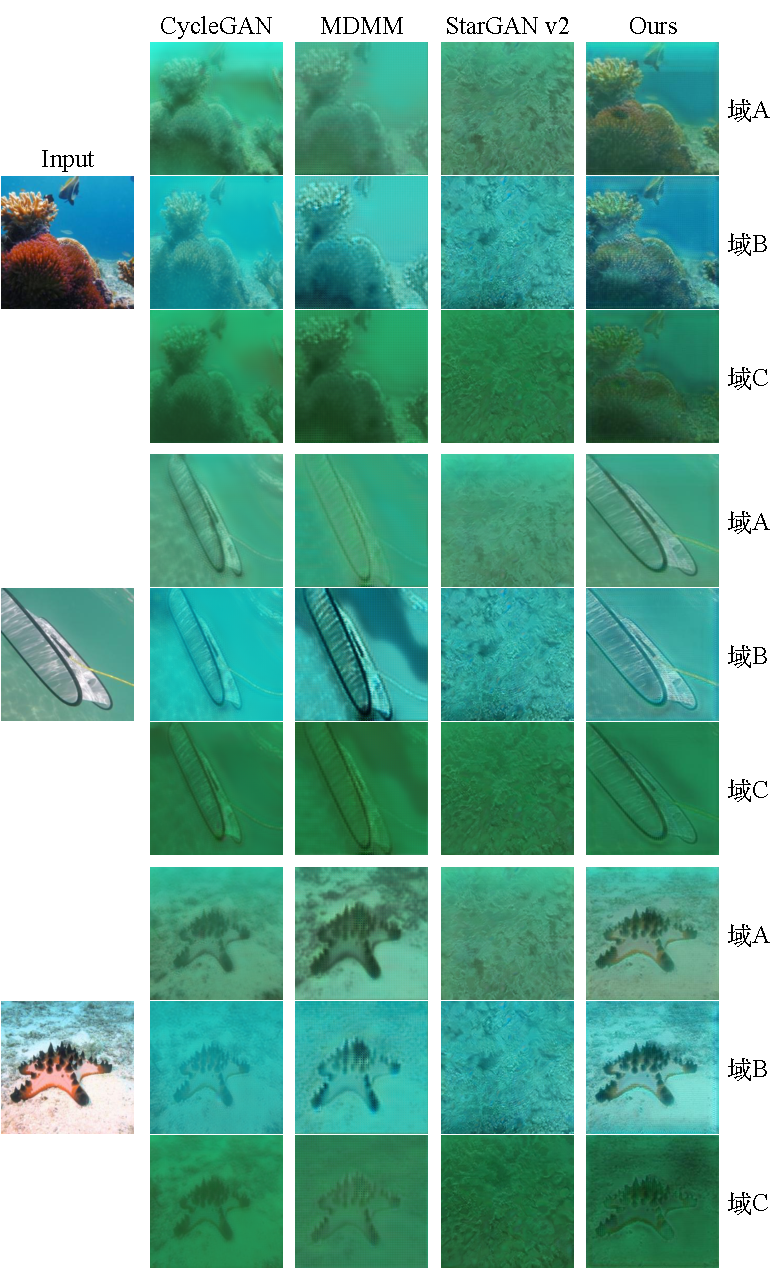
\includegraphics[width=0.95\textwidth]{figures/comparison_domain_ruie.pdf}
  \caption{在RUIE数据集上,基准方法和我们提出的方法在多样式翻译任务结果比较。}
  \label{fig:comparison_domain_ruie}
\end{figure}

图~\ref{fig:comparison_domain_ruie}展示了不同方法在RUIE数据集上的定性结果对比。左边第一列表示模型输入图像,右边每列代表标注方法对应的结果。域$A$代表蓝绿色具有一定浑浊度的域,域$B$代表蓝色水质域,域$C$代表绿色水质域。CycleGAN翻译结果在水质颜色和浑浊度上能接近于真实域内结果,域内内容信息保存完整,缺点在于不能同时实现多个域的翻译。MDMM方法翻译结果在颜色信息上学习基本完整,但是视觉上全局都会有网格样式,导致生成结果内容不够细腻,真实性较差。StarGAN v2翻译后,丢失掉图像中的内容信息,只学到多域的风格信息,推断这是由于输入到多个生成域之间内容差距较大造成的。如图~\ref{fig:ruie_dataset},输入图像来自EUVP数据集,有明显的内容信息,而翻译域是RUIE数据集中多种水质样式域,其中内容不明显。本工作中提出方法的翻译结果,每个域都可以看出明显的对应水质样式区别,内容信息可以保存完整,近处内容颜色信息得到保留,真实性较高。

\begin{figure}
    \centering
  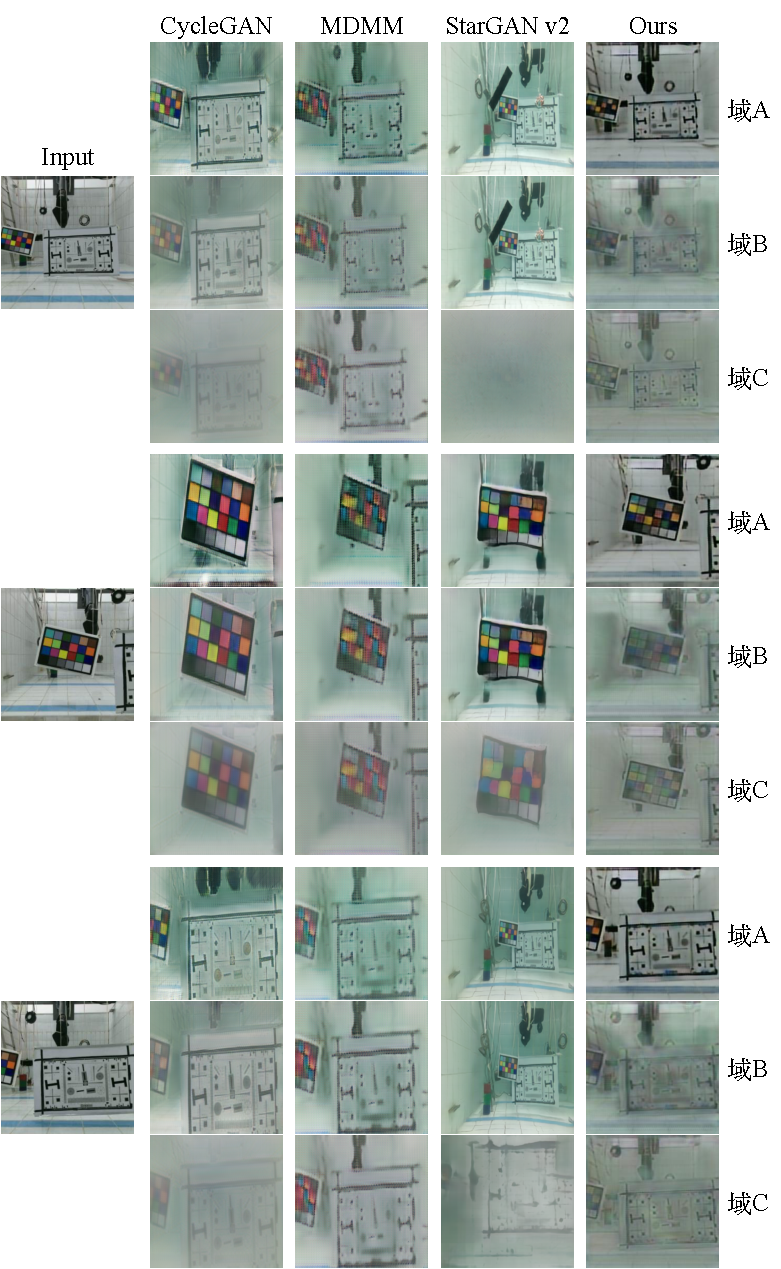
\includegraphics[width=0.95\textwidth]{figures/comparison_domain_uvb.pdf}
  \caption{在UVB 2017数据集上,基准方法和我们提出的方法在多样式翻译任务结果比较。}
  \label{fig:comparison_domain_uvb}
\end{figure}

图~\ref{fig:comparison_domain_uvb}展示了基准方法和我们方法在UVB 2017数据集上的定性结果比较。左边第一列表示模型输入图像,右边每列代表标注方法对应的结果。域$A$,域$B$和域$C$分别为浑浊度不同的三个域,从$A$到$C$浑浊度依次增强。CycleGAN翻译结果,浑浊度变化接近真实样本,内容保存完整,颜色信息得到保留,CycleGAN问题是无法同时生成多个域的结果。MDMM翻译结果,浑浊度变化不太明显,在颜色上有轻微变化,但是内容损失较为严重,内容出现缺损,且有网格状出现。StarGAN v2翻译过程中会改变目标域图像的内容,相同的输入图像转到不同域内时,内容和形状都会发生改变。推断是由于UVB 2017数据集中,不同域之间的内容十分相似,用编码控制生成多域结果时不能很好的通过编码只学到域本身的样式内容。本工作中提出方法的翻译结果能保留完整的内容信息,且浑浊度也有明显的变化。

\begin{figure}
    \centering
  \includegraphics[width=\textwidth]{figures/comparison_domain_uwcnn.pdf}
  \caption{在UWCNN数据集上,基准方法和我们提出的方法在多样式翻译任务结果比较。}
  \label{fig:comparison_domain_uwcnn}
\end{figure}

图~\ref{fig:comparison_domain_uwcnn}展示了基准方法和我们方法在UWCNN数据集上的定性结果对比。左边第一列表示模型输入图像,右边每列代表标注方法对应的结果。域$A$,域$B$,域$C$和域$D$分别表示UWCNN数据集中,近海四种水类型域。通过对比结果我们可以看到,CycleGAN翻译结果,内容清晰,仅样式发生改变,非常接近真实样本数据。MDMM翻译结果,除了会出现网格状样式外,在UWCNN数据集上内容保持完整,样式变化接近真实样本数据。StarGAN v2翻译结果,在该数据集上内容损失严重,内容细节模糊,轮廓扭曲,风格样式学习比较一致。本工作提出方法的翻译结果内容保持完整,风格样式变化一致,结果真实性较高。

\subsection{定量结果分析}
真实性定量指标FID结果如表格~\ref{tab:ruie_domain_fid},表格~\ref{tab:uvb_domain_fid}和~\ref{tab:uwcnn_domain_fid}所示。在图像FID质量分析中,我们对比了能完成水下图像多种样式域翻译的方法CycleGAN、MDMM、StarGAN v2基准方法,在RUIE、UVB 2017、UWCNN数据集上分别进行了测评。通过用FID指标,能够客观的评价各种方法的生成结果。

\begin{table*}[ht]
\centering
\caption{在RUIE数据集上,基准方法和我们方法的真实性FID定量比较。}
  \begin{tabular}{c|ccccccc}
    \hline\noalign{\smallskip}
    FID$\downarrow$ & CycleGAN & MDMM & StarGAN v2 & Ours \\
    \noalign{\smallskip}\hline\noalign{\smallskip}
    Input$\rightarrow$域A & 105.2800 & 154.0302 & 221.6996 & \textbf{82.8535}  \\
    Input$\rightarrow$域B & \textbf{127.3358} & 165.2080 & 160.4444 & 132.0970  \\
    Input$\rightarrow$域C & 99.8060 & 132.0193 & 201.7589 & \textbf{78.8587}  \\
    \noalign{\smallskip}\hline
  \end{tabular}
  \label{tab:ruie_domain_fid}
\end{table*}

\begin{table*}[ht]
\centering
\caption{在UVB 2017数据集上,基准方法和我们方法的真实性FID定量比较。}
  \begin{tabular}{c|ccccccc}
    \hline\noalign{\smallskip}
    FID$\downarrow$ & CycleGAN & MDMM & StarGAN v2 & Ours \\
    \noalign{\smallskip}\hline\noalign{\smallskip}
    Input$\rightarrow$域A & 231.2559 & 308.1764 & 132.5135 & \textbf{123.4455}  \\
    Input$\rightarrow$域B & \textbf{203.3703} & 277.9446 & 261.4843 & 249.0746  \\
    Input$\rightarrow$域C & \textbf{137.9410} & 249.9113 & 203.4555 & 186.2838  \\
    \noalign{\smallskip}\hline
  \end{tabular}
  \label{tab:uvb_domain_fid}
\end{table*}

\begin{table*}[ht]
\centering
\caption{在UWCNN数据集上,基准方法和我们方法的真实性FID定量比较。}
  \begin{tabular}{c|ccccccc}
    \hline\noalign{\smallskip}
    FID$\downarrow$ & CycleGAN & MDMM & StarGAN v2 & Ours \\
    \noalign{\smallskip}\hline\noalign{\smallskip}
    Input$\rightarrow$域A & 141.4799 & 213.1867 & 216.8333 & \textbf{120.0408}  \\
    Input$\rightarrow$域B & 132.0554 & 167.2517 & 168.5740 & \textbf{116.5354}  \\
    Input$\rightarrow$域C & 116.4376 & 158.9736 & 150.5446 & \textbf{98.0187}  \\
    Input$\rightarrow$域D & \textbf{72.5141}  & 136.5694 & 114.0044 & 72.6410  \\
    \noalign{\smallskip}\hline
  \end{tabular}
  \label{tab:uwcnn_domain_fid}
\end{table*}

表格~\ref{tab:ruie_domain_fid},表格~\ref{tab:uvb_domain_fid}和~\ref{tab:uwcnn_domain_fid}中可以看出,CycleGAN和本工作中提出的方法在真实性FID的值处于最低,可以取得具有真实性的最佳结果。尽管CycleGAN在真实性上优于其他基准方法,但是其基于循环一致的网络限制了它不能一次训练实现多域的翻译任务,对于多域翻译任务无法完成。

\begin{table}[htp]
  \centering
  \caption{RUIE数据集上,UCIQE和UIQM定量指标比较。}
    \begin{tabular}{c|c|cc}
    \toprule
    \multicolumn{2}{c|}{} & \multicolumn{1}{c}{UCIQE} & UIQM \\
    \midrule
    \multirow{3}[2]{*}{Real} & Input$\rightarrow$域A & 0.4037$\pm$0.0321 & 2.1390$\pm$0.6176 \\
                             & Input$\rightarrow$域B & 0.4477$\pm$0.0592 & 3.6913$\pm$0.9274 \\
                             & Input$\rightarrow$域C & 0.3820$\pm$0.0333 & 2.2831$\pm$0.5473 \\
    \midrule
    \multirow{3}[2]{*}{CycleGAN} & Input$\rightarrow$域A & 0.4115$\pm$0.0297& 4.0026$\pm$0.3299 \\
                                 & Input$\rightarrow$域B & \textbf{0.4475$\pm$0.0606} &4.7208$\pm$0.5163 \\
                                 & Input$\rightarrow$域C & \textbf{0.3825$\pm$0.0207} &4.0671$\pm$0.2728  \\
    \midrule
    \multirow{3}[2]{*}{MDMM} & Input$\rightarrow$域A & 0.3709$\pm$0.0330 & 4.3429$\pm$0.2728 \\
          & Input$\rightarrow$域B & 0.4335$\pm$0.0439 & 4.7322$\pm$0.2723 \\
          & Input$\rightarrow$域C & 0.3608$\pm$0.0270 & 4.0594$\pm$0.2134 \\
    \midrule
    \multirow{3}[2]{*}{StarGAN v2} &Input$\rightarrow$域A & 0.3553$\pm$0.0058 & 4.2261$\pm$0.2611 \\
          & Input$\rightarrow$域B & 0.3545$\pm$0.0103 & 4.7629$\pm$0.1706 \\
          & Input$\rightarrow$域C & 0.3226$\pm$0.0044 & 4.4751$\pm$0.1607 \\
    \midrule
    \multirow{3}[2]{*}{Our} & Input$\rightarrow$域A & \textbf{0.3999$\pm$0.0362} & \textbf{3.8744$\pm$0.3965} \\
          & Input$\rightarrow$域B & 0.4004$\pm$0.0502 & \textbf{4.3901$\pm$0.4917} \\
          & Input$\rightarrow$域C & 0.3663$\pm$0.0252 & \textbf{4.0515$\pm$0.4076} \\
    \bottomrule
    \end{tabular}%
  \label{tab:underwater_matric_ruie}%
\end{table}%

表格~\ref{tab:underwater_matric_ruie}所示是本工作方法和基准方法在RUIE数据集上的UCIQE和UIQM定量比较结果。表格中可以看出,CycleGAN在$B$域和$C$域翻译可以得到最接近真实样本的结果。除此外,本工作中提出的方法在UCIQE和UIQM指标上都可以得到最接近样本的测评结果,说明我们的方法在RUIE数据集上合成结果具有足够的真实性,最接近真实样本分布。

\begin{table}[htp]
  \centering
  \caption{UVB 2017数据集上,UCIQE和UIQM定量指标比较。}
    \begin{tabular}{c|c|cc}
    \toprule
    \multicolumn{2}{c|}{} & \multicolumn{1}{c}{UCIQE} & UIQM \\
    \midrule
    \multirow{3}[2]{*}{Real} & Input$\rightarrow$域A & 0.4784$\pm$0.0295 & 1.2160$\pm$0.1068 \\
                             & Input$\rightarrow$域B & 0.4023$\pm$0.0600 & 0.7922$\pm$0.2731 \\
                             & Input$\rightarrow$域C & 0.3316$\pm$0.0515 & 0.5776$\pm$0.2575 \\
    \midrule
    \multirow{3}[2]{*}{CycleGAN} & Input$\rightarrow$域A & \textbf{0.4776$\pm$0.0257} & 4.3455$\pm$0.1228 \\
                                 & Input$\rightarrow$域B & 0.3740$\pm$0.0354 & 3.4867$\pm$0.3025 \\
                                 & Input$\rightarrow$域C & 0.3046$\pm$0.0277 & 2.9639$\pm$0.2224  \\
    \midrule
    \multirow{3}[2]{*}{MDMM} & Input$\rightarrow$域A & 0.4471$\pm$0.0311 & 4.3429$\pm$0.2728 \\
          & Input$\rightarrow$域B & 0.3888$\pm$0.0291 & 3.9375$\pm$0.1892 \\
          & Input$\rightarrow$域C & 0.3733$\pm$0.0317 & 3.8126$\pm$0.2193 \\
    \midrule
    \multirow{3}[2]{*}{StarGAN v2} &Input$\rightarrow$域A & 0.4586$\pm$0.0229 & 3.9157$\pm$0.1061 \\
          & Input$\rightarrow$域B & 0.3769$\pm$0.0576 & 3.2742$\pm$0.2138 \\
          & Input$\rightarrow$域C & 0.3235$\pm$0.0507 & 2.9694$\pm$0.1863 \\
    \midrule
    \multirow{3}[2]{*}{Our} & Input$\rightarrow$域A & 0.4800$\pm$0.0291 & \textbf{4.0562$\pm$0.1403} \\
          & Input$\rightarrow$域B & \textbf{0.3980$\pm$0.0576} & \textbf{3.1899$\pm$0.3652} \\
          & Input$\rightarrow$域C & \textbf{0.3258$\pm$0.0436} & \textbf{2.7555$\pm$0.2999} \\
    \bottomrule
    \end{tabular}%
  \label{tab:underwater_matric_uvb}%
\end{table}%

表格~\ref{tab:underwater_matric_uvb}所示是本工作方法和基准方法在UVB 2017数据集上的UCIQE和UIQM定量比较结果。表格中可以看出,CycleGAN在$A$域翻译可以得到最接近真实样本的结果。除此外,本工作中提出的方法在UCIQE和UIQM指标上都可以得到最接近样本数据的结果,说明我们的方法在UVB 2017数据集上合成结果具有足够的真实性。

\begin{table}[htp]
  \centering
  \caption{UWCNN数据集上,UCIQE和UIQM定量指标比较。}
    \begin{tabular}{c|c|cc}
    \toprule
    \multicolumn{2}{c|}{} & \multicolumn{1}{c}{UCIQE} & UIQM \\
    \midrule
    \multirow{3}[2]{*}{Real} & Input$\rightarrow$域A & 0.5150$\pm$0.0629 & 1.8952$\pm$0.6678 \\
                             & Input$\rightarrow$域B & 0.4553$\pm$0.0499 & 1.5497$\pm$0.6500 \\
                             & Input$\rightarrow$域C & 0.3812$\pm$0.0369 & 1.2165$\pm$0.6266 \\
                             & Input$\rightarrow$域D & 0.3609$\pm$0.0274 & 0.8709$\pm$0.5150 \\
    \midrule
    \multirow{3}[2]{*}{CycleGAN} & Input$\rightarrow$域A & 0.5494$\pm$0.0444 & 4.5255$\pm$0.4096 \\
                                 & Input$\rightarrow$域B & \textbf{0.4789$\pm$0.0381} & 4.3994$\pm$0.4449 \\
                                 & Input$\rightarrow$域C & \textbf{0.4011$\pm$0.0333} & 4.2937$\pm$0.4344 \\
                                 & Input$\rightarrow$域D & \textbf{0.3676$\pm$0.0189} & 4.2890$\pm$0.36525 \\
    \midrule
    \multirow{3}[2]{*}{MDMM} & Input$\rightarrow$域A & 0.6234$\pm$0.0322 & 5.0591$\pm$0.2437 \\
          & Input$\rightarrow$域B & 0.5244$\pm$0.0359 & 4.8925$\pm$0.29263 \\
          & Input$\rightarrow$域C & 0.4272$\pm$0.0275 & 4.8056$\pm$0.2918 \\
          & Input$\rightarrow$域D & 0.4238$\pm$0.0219 & 4.8769$\pm$0.2636 \\
    \midrule
    \multirow{3}[2]{*}{StarGAN v2} &Input$\rightarrow$域A & 0.4887$\pm$0.06899 & 4.4896$\pm$0.4803 \\
          & Input$\rightarrow$域B & 0.4172$\pm$0.0579 & 4.2180$\pm$0.5526 \\
          & Input$\rightarrow$域C & 0.3184$\pm$±0.0232 & 3.2936$\pm$0.3978 \\
          & Input$\rightarrow$域D & 0.3272$\pm$0.0135 & 3.3656$\pm$0.3795 \\
    \midrule
    \multirow{3}[2]{*}{Our} & Input$\rightarrow$域A & \textbf{0.5063$\pm$0.5063} & \textbf{3.7514$\pm$0.6967} \\
          & Input$\rightarrow$域B & 0.3674$\pm$0.0469 & \textbf{3.1748$\pm$0.5785} \\
          & Input$\rightarrow$域C & 0.3432$\pm$0.0362 & \textbf{3.0890$\pm$0.6834} \\
          & Input$\rightarrow$域D & 0.3361$\pm$0.0278 & \textbf{2.9932$\pm$0.8089} \\
    \bottomrule
    \end{tabular}%
  \label{tab:underwater_matric_uwcnn}%
\end{table}%

表格~\ref{tab:underwater_matric_uwcnn}所示是本工作方法和基准方法在UWCNN数据集上的UCIQE和UIQM定量比较结果。由表格可以看出,在UCIQE上,CycleGAN在三个域的翻译上都可以得到最好的结果,本工作中提出的方法在UCIQE一个域和UIQM指标上都得到最接近真实样本的结果。由此可见,CycleGAN和我们的方法能够在多域翻译任务上得到最接近真实的结果,CycleGAN无法同时实现多域翻译,在此多域翻译任务上,我们的方法可以成功获得足够真实的合成结果。